\section{Топологические пространства}
\subsection{Основные понятия}
\begin{definition}
    \textit{Метрика} — это функция $\rho(x,y) \to \R$, которая обладает следующими свойствами:
    \begin{enumerate}
        \item $\rho(x,y) \geq 0, \ \rho(x,y) = 0 \Leftrightarrow x = y$;
        \item $\rho(x,y) = \rho(y,x)$;
        \item $\rho(x,z) + \rho(z,y) \geq \rho(x,y)$.
    \end{enumerate}
\end{definition}

\begin{definition}
    Множество $X$ называется \textit{метрическим пространством}, если на нём задана метрика $\rho(x,y): X \times X \to \R$.
\end{definition}

\begin{definition}
    \textit{$\epsilon$-окрестность точки $x_0$} — это множество всех точек $x \in X: \ \rho(x, x_0) < \epsilon$.
\end{definition}

% спасибо Кириллу за конспект курса математического анализа
Из курса математического анализа.
\begin{definition}
    Точка $x \in X \subset A$ называется внутренней точкой множества $X$, если $\exists B_{\epsilon} (x) \subset X$.
\end{definition}

\begin{definition}
    Множество называется открытым, если все его точки — внутренние.
\end{definition}

\begin{definition}
    Множество $A$ называется закрытым, если его дополнение $A \setminus X$ открыто.
\end{definition}

Свойства открытых множеств:
\begin{enumerate}
    \item Пустое множество и само множество $X$ открыты;
    \item Любые объединения открытых множеств открыты;
    \item Конечное пересечение открытых множеств открыто.
\end{enumerate}

%\begin{definition}
%    Множество $X$ называется \textit{топологическим пространством}, если на нём выбран набор его подмножеств $\tau$, которые называются %открытыми и удовлетворяют следующим свойствам:
%    \begin{enumerate}
%        \item $\emptyset, X = \tau$.
%        \item Любые объединения открытых множеств открыты.
%        \item Конечное пересечение открытых множеств открыто.
%    \end{enumerate}
%\end{definition}

\begin{definition}
    Семейство $\tau$ подмножеств некоторого множества $X$, удовлетворяющее условиям 1-3, называется \textit{топологией}.
\end{definition}

\begin{definition}
    Пусть $X$ — произвольное множество и $\tau = \{U_{\alpha}\}$ — некоторое семейство подмножеств множества $X$. Семейство подмножеств $\tau$ называется \textit{топологией}, если оно удовлетворяет следующим условиям:
    \begin{enumerate}
        \item Пустое множество и само множество $X$ принадлежат $\tau$;
        \item Объединение любого семейства множеств из $\tau$ принадлежит $\tau$;
        \item Пересечение любого конечного семейства множеств из $\tau$ также принадлежит $\tau$.
    \end{enumerate}
\end{definition}

\begin{definition}
    Множество $X$ с фиксированной топологией $\tau$ называется \textit{топологическим пространством} и обозначается через $(X, \tau)$. Элементы множества $X$ называются \textit{точками}. Множества из $\tau$ называются \textit{открытыми} в $(X, \tau)$.
\end{definition}

Если $X$ — метрическое пространство, то на нём можно задать топологию, индуцированную метрикой: множество открыто, если любая точка входит в него с некоторым $\epsilon$-шаром (некоторой окрестностью).

[Дополнение вне лекций] Топология, индуцированная метрикой — это топология, в которой открытые множества определяются через $\epsilon$-шары. Таким образом, топология $\tau$ на множестве $X$ задаётся как:
\[\tau = \left\{U \subset X | \ \forall x \in U \ \exists r > 0: B_r(x) \subset U\right\}\]

\begin{example}
    \begin{enumerate}
        \item $\emptyset, X$, других нет — \textit{тривиальная топология}.
        \item Семейство $\tau$ состоит из всех подмножеств множества $X$ — \textit{дискретная топология}.
    \end{enumerate}
\end{example}

\begin{definition}
    Множество $A$ топологического пространства $X$ называется \textit{замкнутым}, если его дополнение $X \setminus A$ открыто.
\end{definition}

\begin{definition}
    Пусть $X$ — топологическое множество, $x_0 \in X$. \textit{Окрестностью точки $x_0$} назовём любое открытое множество, содержащее эту точку.
\end{definition}

\begin{statement}
    Множество $A$ топологического пространства $X$ открыто $\Leftrightarrow$ $\forall x_0 \in A \ \exists U_{x_0} \in \tau: x_0 \ \in U_{x_0} \subset A$
\end{statement}
\begin{proof}
    $\underline{\Longrightarrow}$ Пусть $A$ открыто, $x_0$ — точка $A$, тогда $U_{x_0} = A$. \\
    $\underline{\Longleftarrow}$ Возьмём $x \in U_x \subset A$, где $U_x$ открыты ($\in \tau$).
    Рассмотрим $\cup_{x \in A} U_x = U$, где $U$ открыто, т.к. все $U_x$ открыты.
    При этом $A \subset U$ и $U \subset A \Rightarrow U = A \Rightarrow A$ открыто.
\end{proof}

\subsection{Непрерывность}
% украдено.
\begin{definition} Обратимся к курсу математического анализа.
    Пусть $D_f$ — область определения $f(x),\ x_0\in D_f$. Если 
    \[\forall \epsilon>0\ \exists\ \delta_{\epsilon}>0,\ \forall x\in B_{\delta_{\epsilon}}(x_0)\cap D_f: |f(x)-f(x_0)|<\epsilon,\] 
    то $f(x)$ называется \textit{непрерывной} в точке $x_0$. \\
    $$f: X \to Y \ \forall B_{\epsilon}(f(x_0)) \ \exists B_{\delta}(x_0): f(B_{\delta}(x_0)) \subset B_{\epsilon}(f(x_0))$$ — в терминах окрестностей.
\end{definition}

\begin{definition}
    Отображение $f: X \to Y$ топологии пространств $X$ и $Y$ \textit{непрерывно}, если $\forall x_0 \in X$ и для любой окрестности $\delta$ точки $f(x_0)$ существует окрестность точки $x_0$ такая, что $f(B(x_0)) \subset B_{\delta} (f(x_0))$.
\end{definition}

\begin{statement}
    Отображение $f$ двух топологических пространств непрерывно $\Leftrightarrow$ прообраз любого открытого множества открыт.
\end{statement}
\begin{proof}
    $\underline{\Longrightarrow}$ $f: X \to Y$. Пусть $A \subset Y$ открыто. Рассмотрим $f^{-1}(A)$. Пусть $x_0 \in f^{-1}(A) \Rightarrow \exists U$ — открытое: $f(U) \subset A \Rightarrow U \subset f^{-1}(A)$. \\
    $\underline{\Longleftarrow}$ Пусть прообраз любого множества открыт. Пусть $x_0 \in X \Rightarrow f(x_0) \in Y$. Возьмём $V \subset Y$, которое будет открыто. $f(x_0) \in V \Rightarrow f^{-1}(V)$ — открытое множество и $x_0 \in f^{-1}(V) \Rightarrow U := f^{-1}(V)$.
\end{proof}

%Другие способы задания топологии:
\subsection{Способы задания топологии}
\begin{enumerate}
    \item Топология на подмножестве: \\
    Пусть $X$ — топологическое пространство. $$X_0 \subset X, \ U \in \tau(X) \Rightarrow \ U \cap X_0 \in \tau(X_0).$$
    \item $f: X \to Y$, $Y$ — топологическое пространство, $f$ — произвольное отображение. Тогда открытые множества на $X$ — прообразы открытых на $Y$, то есть:
    \[\tau_X = \left\{f^{-1}(U) | \ U \in \tau_Y\right\}\]
\end{enumerate}

\begin{remark}[Дополнение с лекции №2]
    Топология на $Y$ порождается отображением $f$: множество открыто, если его прообраз открыт.
\end{remark}

\subsection{Гомеоморфизм}
\begin{definition}
    Топологические пространства $X$ и $Y$ называются \textit{гомеоморфными}, если между ними существует непрерывная биекция $f: X \to Y$, которая и называется \textit{гомеоморфизмом}, такая, что отображение $f^{-1}$ также непрерывно.
\end{definition}

%Возвращаемся к гомеоморфизму.
% Из второй лекции
% \begin{example}
%     Интервал гомеоморфен вещественной прямой $\R$: можно задать гомеоморфизм между окружностью и прямой, гомеоморфизм между отрезком и прямой строится «растягиванием окружности».
% \end{example}

\begin{example}
    Окружность с выколотым полюсом и прямая гомеоморфны (см.рис. \ref{fig:c1.1}).
\end{example}

\begin{figure}
    \centering
    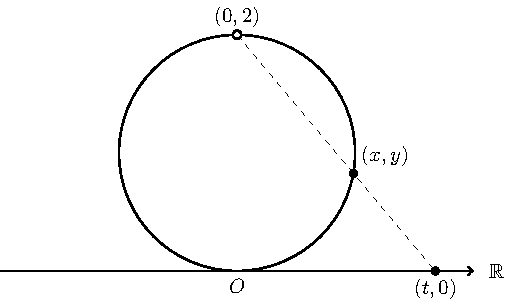
\includegraphics{images/c1.1.pdf}
    \caption{Окружность с выколотым полюсом и прямая гомеоморфны.}
    \label{fig:c1.1}
\end{figure}


\subsection{Связность}
\begin{definition}
    Топологическое пространство $X$ называется \textit{связным}, если не существует двух открытых непустых непересекающихся множеств $A$ и $B$ таких, что $X = A \cup B$.
\end{definition}

\begin{statement}
    Отрезок вещественной прямой в стандартной топологии связен.
\end{statement}
\begin{proof}
    От противного. Пусть отрезок несвязен. $\exists A, B \subset \R: \ [a, b] = A \cup B, \ A \cap B = \emptyset$, где $A, B$ — открытые множества. Пусть $\alpha \in A$, тогда $[a, \alpha) \subset A$ (т.к. A открыто). Рассмотрим $\alpha_0 = \sup{\alpha}: [a, \alpha) \subset A$. \\
    Пусть $\alpha_0 \in A$, тогда:
    \begin{enumerate}
        \item $\alpha_0 = b \Rightarrow B = \emptyset$ — противоречие.
        \item $\alpha_0 < b \Rightarrow \alpha_0$ входит в $A$ с окрестностью $\Rightarrow$ существует $(\alpha_0 - \epsilon, \alpha_0 + \epsilon) \in A \Rightarrow \alpha_0$ — не супремум — противоречие.
    \end{enumerate}
\end{proof}

% конец первой лекции